%%%%%%%%%%%%%%%%%%%%%%%%%%%%%%%%%%%%%%%%%%%%%%%%%%%%%%%%%%%%%%%%%%%%%%%%%%%%%%%%
%2345678901234567890123456789012345678901234567890123456789012345678901234567890
%        1         2         3         4         5         6         7         8

\documentclass[letterpaper, 10 pt, conference]{ieeeconf}  % Comment this line out
                                                          % if you need a4paper
%\documentclass[a4paper, 10pt, conference]{ieeeconf}      % Use this line for a4
                                                          % paper
\IEEEoverridecommandlockouts                              % This command is only
                                                          % needed if you want to
                                                          % use the \thanks command
%\overrideIEEEmargins
% See the \addtolength command later in the file to balance the column lengths
% on the last page of the document

% The following packages can be found on http:\\www.ctan.org
\usepackage{cite}
\usepackage{amsmath,amssymb,amsfonts}
\usepackage{algorithmic}
\usepackage{graphicx}
\usepackage{textcomp}
\usepackage{xcolor}

\title{\LARGE \bf
Outlier Detection for ARM Data
}

\author{Yuping Lu$^{1}$, Jitendra Kumar$^{2}$ and Michael A. Langston$^{1}$% <-this % stops a space
\thanks{$^{1}$University of Tennessee, Knoxville, TN, USA}%
\thanks{$^{2}$Oak Ridge National Laboratory, Oak Ridge, TN, USA}%
}

\begin{document}
\maketitle
\thispagestyle{empty}
\pagestyle{empty}

%%%%%%%%%%%%%%%%%%%%%%%%%%%%%%%%%%%%%%%%%%%%%%%%%%%%%%%%%%%%%%%%%%%%%%%%%%%%%%%%
\begin{abstract}

Outliers are common in ARM data. These outliers could be either an instrument
failure or extreme weather event. Multiple methods are available to detect 
these outliers from the huge ARM datasets. We combined Pearson Correlation Coefficient, 
Singular Spectrum Analysis and K-means methods together as a whole framework
to track down these outliers. Compared to the current outliers recorded in the
DQR database, our results showed this framework is promising.

\end{abstract}


%%%%%%%%%%%%%%%%%%%%%%%%%%%%%%%%%%%%%%%%%%%%%%%%%%%%%%%%%%%%%%%%%%%%%%%%%%%%%%%%
\section{Introduction}
We will use this section to introduce the background of outlier detection for 
time series data. \cite{gupta2014outlier} 

The Atmospheric Radiation Measurement (ARM) user facility was founded by the U.S. 
Department of Energy (DOE) in 1989 \cite{ARM}. Since then, its aim is to be the 
platforms for the observation and study of Earth's climate. Huge ARM datasests 
are generated and stored in ARM data center daily. And outliers are pretty common 
in these datasets. Currently, these datasets are checked manually and outliers 
are stored in Data Quality Report (DQR) database to be fixed.

\section{Datasets}
ARM data center gathers data from multiple data sources. It ranges from \textit{Atmospheric 
Profiling} to \textit{Satellite Observations}. All these data are measured at different 
locations using different instruments. Each instrument may only work on a specified
time range. For the raw netcdf dataset collected from each instrument, it contains
multiple variables. In this paper, we only tested Surface Meteorology Systems (MET)
data collected from the Southern Great Plains (SGP). There were total 24 instruments
in SGP area and we chose 5 typical variables which are \textit{temp\_mean}, 
\textit{vapor\_pressure\_mean}, \textit{atmos\_pressure}, 
\textit{rh\_mean} and \textit{wspd\_arith\_mean} from multiple variables. Table 1 
contains the detail of these datasets.

\begin{table}[ht]
\caption{SGPMET datasets tested}
\label{tab:template}
\centering
\begin{tabular}{|l|c|c|c|c|c|c|c|c|}
\hline
Instrument & E1 & E3 & E4 & E5 & E6 & E7\\
Begin Year & 1996 & 1997 & 1996 & 1997 & 1997 & 1996\\
End Year & 2008 & 2008 & 2010 & 2008 & 2010 & 2011\\
\hline
Instrument & E8 & E9 & E11 & E13 & E15 & E20\\
Begin Year & 1994 & 1994 & 1996 & 1994 & 1994 & 1994\\
End Year & 2008 & 2017 & 2017 & 2017 & 2017 & 2010\\
\hline
Instrument & E21 & E24 & E25 & E27 & E31 & E32\\
Begin Year & 2000 & 1996 & 1997 & 2004 & 2012 & 2012\\
End Year & 2017 & 2008 & 2001 & 2009 & 2017 & 2017\\
\hline
Instrument & E33 & E34 & E35 & E36 & E37 & E38\\
Begin Year & 2012 & 2012 & 2012 & 2012 & 2012 & 2012\\
End Year & 2017 & 2017 & 2017 & 2017 & 2017 & 2017\\
\hline
\end{tabular}
\end{table}

%var_names = ['temp_mean', 'vapor_pressure_mean', 'atmos_pressure', 'rh_mean', 'wspd_arith_mean']

\section{Methodology}
Mention methods we used in this paper and how do we preprocess the data.

\subsection{Pearson Correlation Coefficient} 
PCC goes here \cite{pearson1895note}.

% add detail explanation about the figure later
\subsection{Singular Spectrum Analysis}
SSA goes here \cite{golyandina2013singular, alexandrov2008method}.
\begin{figure*}[ht]
    \centering
    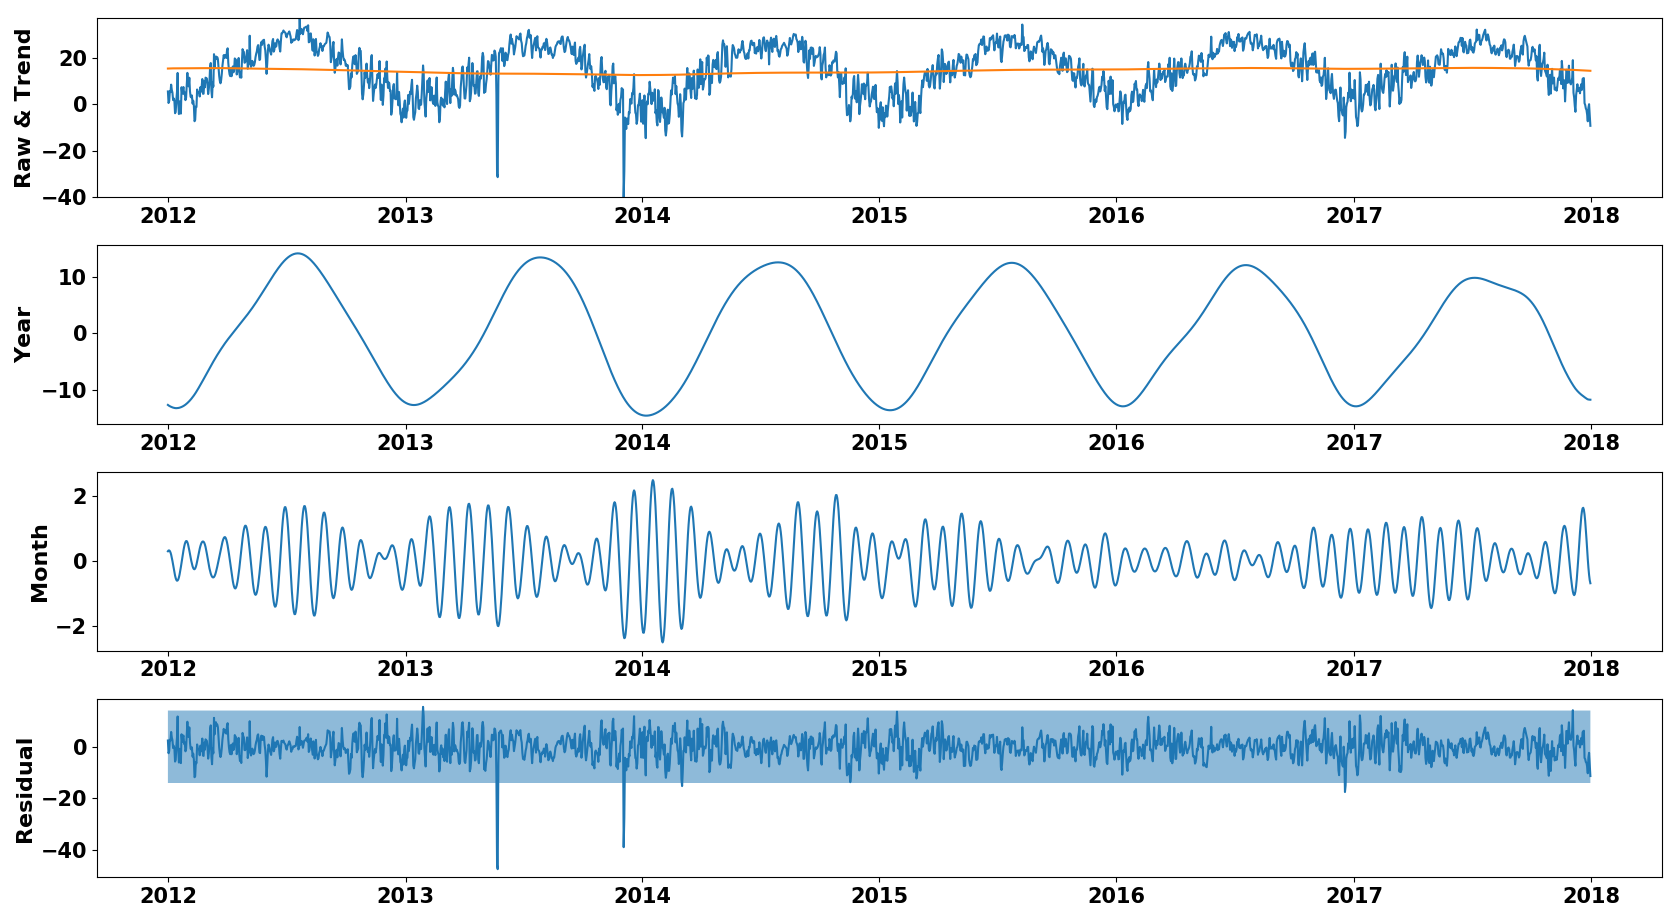
\includegraphics[width=\textwidth]{E33.png}
    \caption{Example of SSA application on ARM data. E33 temp\_mean data full 
    decomposition.}
    \label{fig:sample_figure}
\end{figure*}

\subsection{K-means}
k-means goes here \cite{hartigan1979algorithm}.


\section{Results and Discussion}
Results and pics go here. Comparison metric: DQR database. Add precision and 
recall result here \cite{perry1955machine}.


\section{Conclusions}
We presented a combined model to detect outliers for ARM data. Future work: 
ML and tried methods working on multiple instruments multiple sites \cite{phillips2015graph}.

%\addtolength{\textheight}{-12cm}  % This command serves to balance the column lengths
                                  % on the last page of the document manually. It shortens
                                  % the textheight of the last page by a suitable amount.
                                  % This command does not take effect until the next page
                                  % so it should come on the page before the last. Make
                                  % sure that you do not shorten the textheight too much.

%%%%%%%%%%%%%%%%%%%%%%%%%%%%%%%%%%%%%%%%%%%%%%%%%%%%%%%%%%%%%%%%%%%%%%%%%%%%%%%%
\section*{Acknowledgment}
This research was supported by the Atmospheric Radiation Measurement (ARM) user 
facility, a U.S. Department of Energy (DOE) Office of Science user facility 
managed by the Office of Biological and Environmental Research.


\bibliography{main} 
\bibliographystyle{IEEEtran}


\end{document}